

\chapter{Collapse and dynamical evolution}


In this chapter, we let the \HubLem models evolve and undergo violent relaxation. We compare their dynamical evolution with that of cold uniform models. We investigate the evolution of the structure and global mass segregation.

\minitoc

\section{The simulations}
\label{Sec:3_simulations}

\subsection{Description of the models}

The \HubLem fragmented system is subvirial by construction. The configuration we took as a reference is the apex of the expansion: the kinetic energy initially injected in the expansion has been converted into potential energy through expansion or converted to transversal motion by two-body interaction. If the model is left to evolve further, it collapses, violently relaxing to reach a quasi-equilibrium state, resembling a Plummer or King model.

In the present chapter, simulations will use the fully fragmented state of Hubble models as initial conditions for the subsequent dynamical evolution. Observational clues point to  collapsing and violently relaxing clusters. For example, \cite{Cottaar2015} find IC 348, a young (2-6 Myr) cluster, to be both survirial and with a convergent velocity field, consistent with infalling motion. Our models undergo dry collapse with no gas, while real objects such as IC 348 still contain residual gas. The scenario of our simulations is an idealized situation: clearly if there was residual gas between the clumps and it was evacuated through stellar feedback, both the clump merger rate and the depth of the potential achieved during relaxation would be affected. As a limiting case, rapid gas removal may lead to total dissolution (see for instance \citealt{Moeckel2012} and \citealt{Fujii2016}). In the current situation, all clumps will merge. 


The numerical integration were done once more with the NBODY6 integrator with the same computational units. For comparison purposes, we also performed simulations of cold uniform spheres, a configuration which has been extensively used  in the past (e.g.,\citealt{Theis1999,Boily2002,Barnes2009,Caputo2014,Benhaiem2015}) and one that minimises the level of fragmentation and mass segregation in the on-set of collapse. The models are referenced as Rh100, Rh20,Ru100 and Ru20 in Table~\ref{Tab:2_models}. The aspects of Rh20 and Ru20 during collapse are shown on Fig~\ref{Fig:3_collapse}. Note the deeper collapse of the uniform system.

 We focus here on models with a mass function from 0.35$\Mo$ to 20$\Mo$ and 15000 stars, a compromise value for rich open clusters that should allow us to identify clearly collisional effects and trends with time, and ease comparison with the recent study by \cite{Caputo2014} where most calculations are performed with that sampling. We let both Hubble-fragmented and uniform sphere evolve up to 40 H.u. 





\begin{figure}
\begin{center}
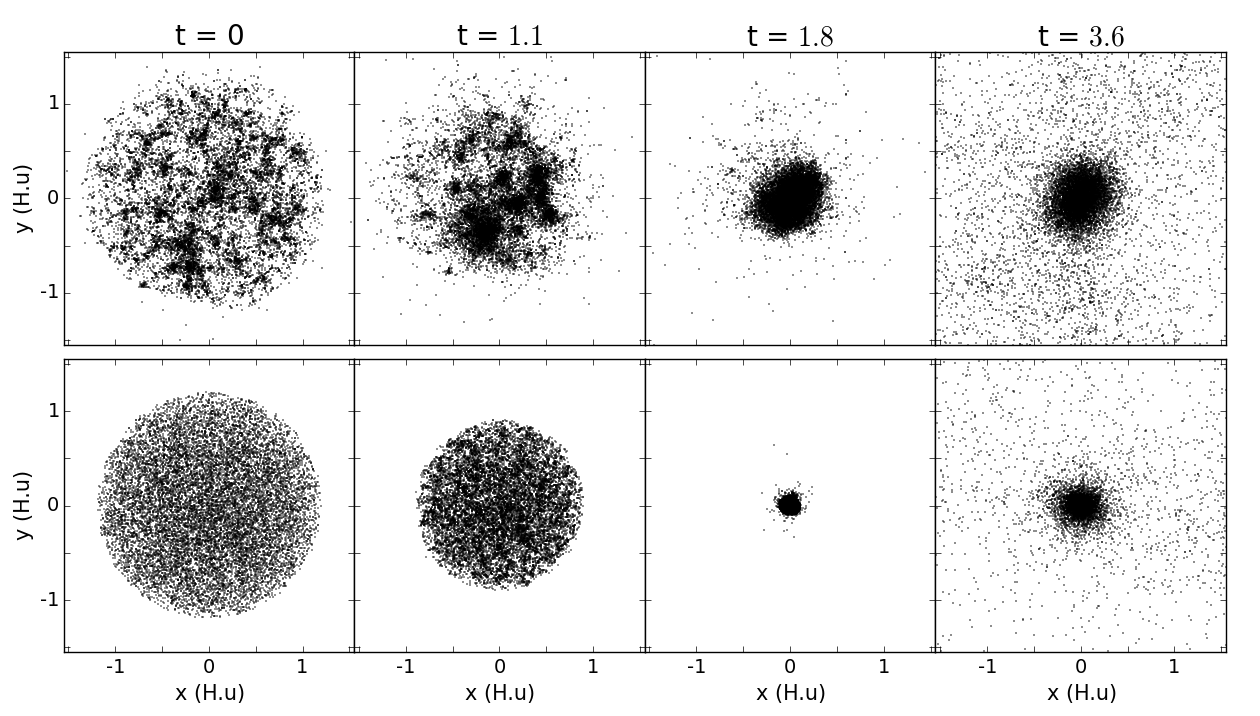
\includegraphics[width=\textwidth]{Figures/3_collapse}
\caption[Stages of collapse for HL fragmented and uniform models]{Aspects of both Hubble (top panels) and uniform (bottom panels) systems throughout the collapse. The epochs shown are, from left to right: initial conditions; half-collapse; point of deepest collapse; direct aftermath of collapse. The times are in H\'enon units.}
\label{Fig:3_collapse}
\end{center}
\end{figure}


\subsection{Scaling to physical units}
\label{Sec:3_Scaling}
Before discussing the results, it is useful to translate the units of computation to physical scales. This is important if we want to discuss the state of the systems using one and the same physical time, such that the hypothesis of no stellar evolution holds.
To do so, we compute the free-fall time of an uniform sphere (a good approximation for fragmented model as well) both in physical units and H\'enon units, which provide a conversion factor. We first have to choose an initial physical length scale for the system by setting $R_h = 1$ pc. With a total system mass of $M = 15\cdot 10^3\, \Mo$, this gives the uniform half-mass volume density 
\begin{equation}
\rho_h = \frac{M/2}{\frac{4}{3}\pi r_h^3}  \simeq 1.8 \cdot10^3 \Mo / pc^3,
\end{equation}
within values typically inferred from observations of clusters.

 The free-fall time of an uniform sphere, obtained from conservation of energy and integration, is expressed as
\begin{equation}
t_{ff} = \sqrt{\frac{3\pi}{32 G \rho_{h	}}}.
\end{equation}
Computing $\rho_{h,\textrm{H\'enon}} \simeq 0.13$, we now compute both values of the free-fall time
\begin{align}
t_{ff} &\simeq 1.5~ t_\Hen\\
	   &\simeq 0.2~ \Myr
\end{align}
which gives: 
\begin{equation}
1 ~ t_\Hen \equiv 0.13~ \Myr = 1.3 \cdot 10^5 \yr .
\end{equation}


Thus by running up to 40 H.u we ensure that the systems evolve for $ \sim  6~\Myr $, about the lifetime of a 50$\Mo$ star. \footnote{For our models with more massive stars, up to 100$\Mo$, these represent only $\sim$ 5\% of the total mass and their removal would not significantly alter the dynamics of the system.}

We now want to evaluate the crossing and relaxation time-scales in such a system, as they were defined in the introduction (\ref{Sub:0_time-scales}), and how they relate to the total duration of the simulation. We could attempt to derive a crossing time for the initial, subvirial state but it would not be representative of the evolution of the system. Instead, the more useful crossing time has to be computed from the equilibrium state achieved. Using the virial theorem and conservation of energy, we derive dynamical time-scales for the equilibrium system. The crossing times is defined as
\begin{equation}
\label{Eq:3_tcr}
t_{cr,eq} = \frac{2 R_{h,eq}}{\sigma_{1d,eq}}.
\end{equation}

From here on, we write the subscript 0 for initial values and no subscript for equilibrium values. To obtain both $R_{h}$ and $\sigma_{1d}$ we start from the total energy of the system. At t=0, velocities are null, all energy is potential energy. It can be computed by integrating from the center to $R_0$. We obtain
\begin{equation}
E_0 = - \frac{3}{5} \frac{G M^2}{R_0}.
\end{equation}
From virial theorem and conservation of energy, we get the following equations at equilibrium
\begin{equation}
\label{Eq:3_energies}
\begin{cases}
2 E_k + E_p &=0\\
E_k + E_p &= E_0
\end{cases} 
\quad
\implies
\quad
\begin{cases}
E_k &= -E_0 = \frac{3}{5} \frac{G M^2}{R_0}\\
E_p &= 2 E_0 = - \frac{6}{5} \frac{G M^2}{R_0}.
\end{cases}
\end{equation}
which can be combined with
\begin{equation}
E_k = \frac{1}{2} M \sigma_{3d}^2 = \frac{3}{2} M \sigma_{1d}^2
\end{equation}
to get
\begin{equation}
\sigma_{1d} = \sqrt{\frac{2 G M}{5 R_0}}.
\end{equation}

As for the half-mass radius at equilibrium, its value is dependant on how concentrated the system is and is not easy to derive. However, numerically obtained King models show that in relaxed systems, there is a consistent relation between $R_h$ and the virial radius $R_v$, defined as 
\begin{equation}
\label{Eq:3_virialradius}
E_p = - \frac{G M^2}{2 R_v},
\end{equation}
that gives 
\begin{equation}
\label{Eq:3_radii}
R_{h,eq} \approx 1.3 \times R_{v,eq}.
\end{equation}

 Combining Eq.~(\ref{Eq:3_energies}),~(\ref{Eq:3_virialradius}) and~(\ref{Eq:3_radii})  it comes
\begin{equation}
R_{h,eq} \approx 0.54 R_0.
\end{equation}


Knowing that $R_0 = 2^{1/3} R_{h,0}$, we now write a good approximation of the crossing time in the relaxed, equilibrium system
\begin{align}
t_{cr}  &\simeq 1.7\frac{R_0^{3/2}}{\sqrt{GM}}\\
        &\simeq 2.4~ t_\Hen\\
	    &\simeq 0.3~ \Myr.
\end{align}

 With $N = 15 000$  we find from (\ref{Eq:0_trel}) a two-body relaxation time-scale

\begin{align}
t_{rel}  &\simeq 324~ t_\Hen\\
	     &\simeq 95~ \Myr
\end{align}

and from (\ref{Eq:0_ms2}), considering a mass range of $m_{max}/\langle m\rangle = 20$, we find a mass-segregation time-scale

\begin{align}
t_{ms}  &\simeq 25~ t_\Hen\\
	    &\simeq 7.5~ \Myr
\end{align}

Our simulations last for far less than a relaxation time, but we expect to see some dynamical mass segregation set in in our models.


\subsection{Removal of the ejected stars}

In the previous section, we considered there was no mass loss during the collapse and relaxation that lead to the equilibrium system. However, a look at the simulations shows this assumption does not hold. Some stars are ejected from the system after the collapse, when the system bounces. These stars are not part of the equilibrium system as they have no influence on the central dynamics.

To investigate the evolution of the central bound system only, we need to isolate and substract the ejected stars. The obvious way to do this would be to compute the stars mechanical energies and to remove all stars with positive energy. Though this works for a majority of the ejected stars, a subset of them has a marginally negative energy. These register as bound when they are essentially out of the system (far beyond the original system radius). 

To efficiently collect a maximum number of ejected stars, we spotted the time when the potential energy is maximum, when the collapse occurs. We  then identified all stars whose distance to the center increased monotonically from there onwards. The full selection criteria is therefore~:

\begin{equation}
v_r(t) > 0,~\forall t > t_{ff}\quad \textrm{or} \quad  E_\star > 0 , ~\forall t > t_{ff}
\end{equation}
 
This allows a more complete selection of the ejecta.  On Fig.~\ref{Fig:3_DistOrigin} we graph  $|\bold{r}|$  as a function of time for a subset of escapers (shown as red curves) for the uniform collapse model Ru20. The black curves are trajectories for bound stars given for comparison. Some of these bound stars are later ejected from the system due to close interactions, as seen on the figure.

\begin{figure}
\begin{center}
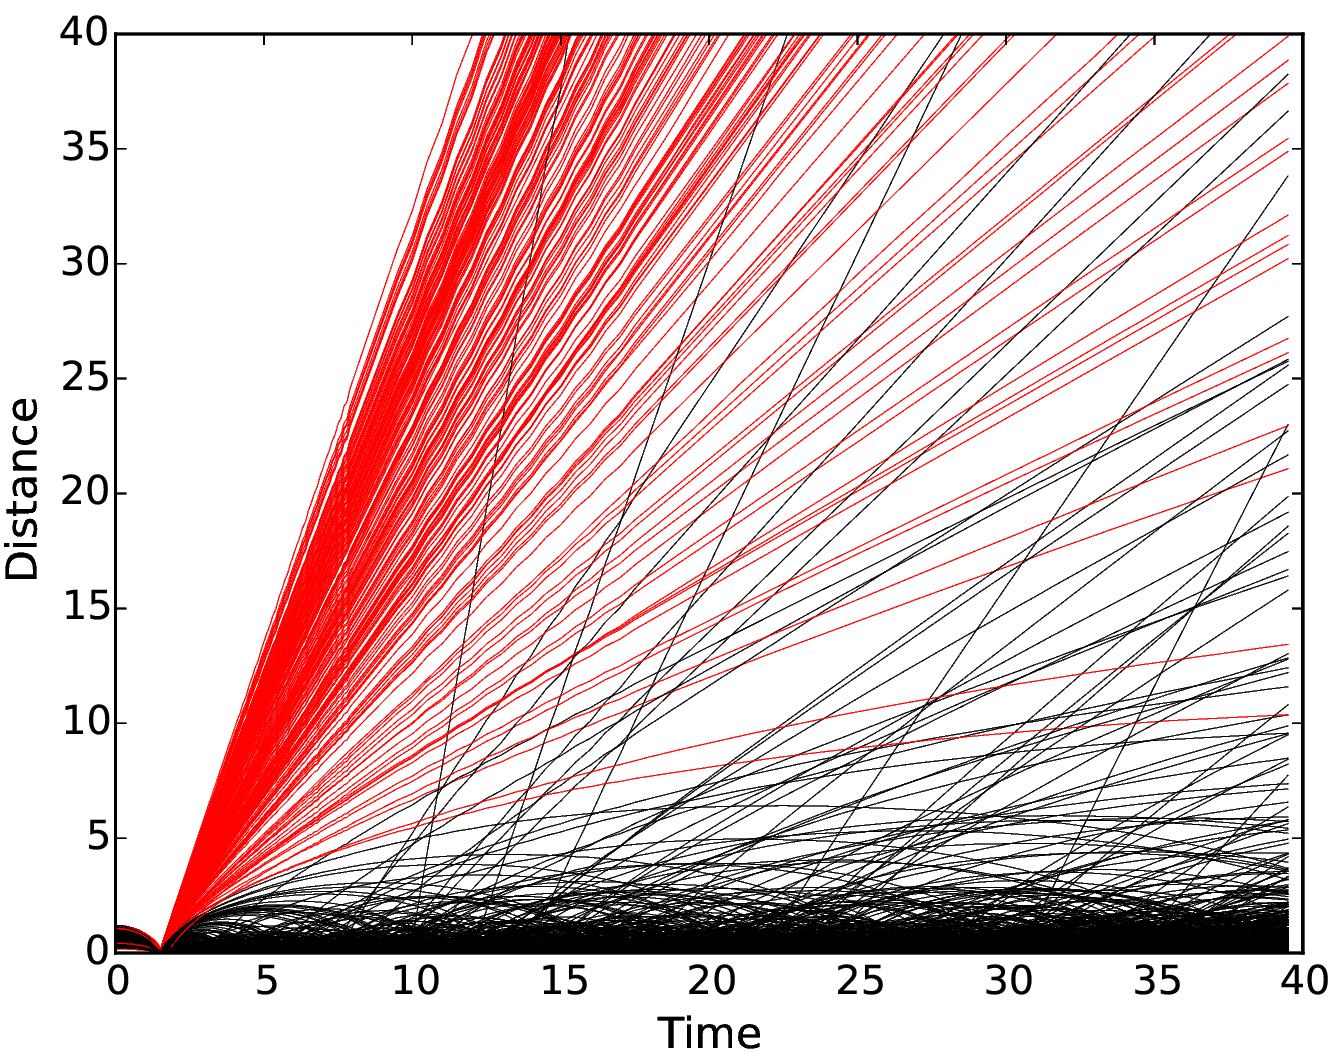
\includegraphics[width=0.7\textwidth]{Figures/3_DistOrigin}
\caption[Distance to origin over time for escapers and bound stars]{Distance to origin for 750 stars from run Ru20 (see Table~\ref{Tab:2_models}). Red lines show the trajectory of stars that are considered ejected according to our criterion.}
\label{Fig:3_DistOrigin}
\end{center}
\end{figure}



  
\section{Collapse and virialisation}
\label{Sec:Collapse}


The constant diffusion of kinetic energy by two-body interaction means that no stellar system ever reaches a steady equilibrium. However we can contrast the time-evolution of two configurations and draw conclusions about their observable properties. 







\begin{figure}
\begin{center}
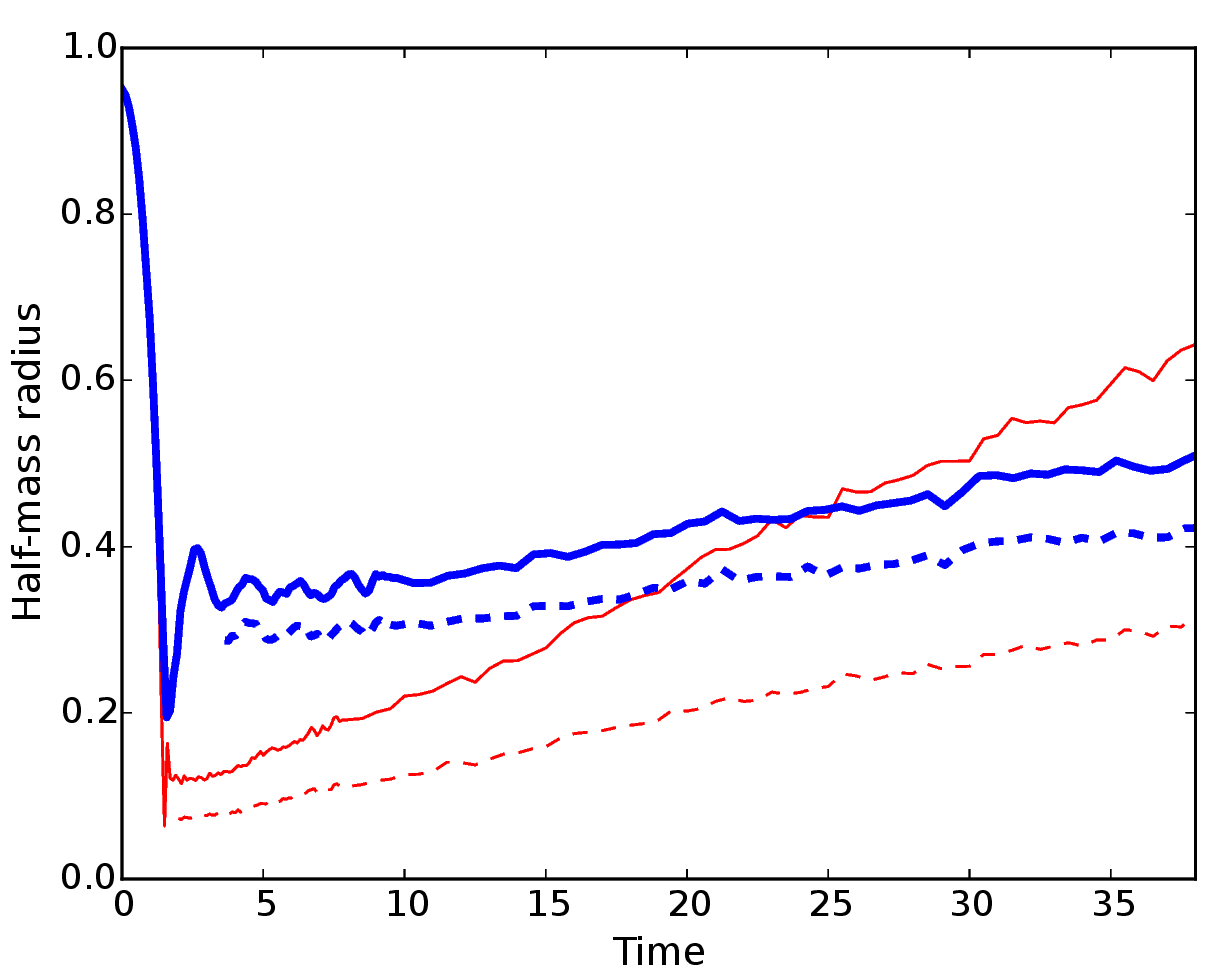
\includegraphics[width=0.7\textwidth]{Figures/3_Rhm_global}
\caption[Half-mass radius as function of time for both HL fragmented and uniform model]{Half-mass radius as function of time for two systems undergoing collapse~: a uniform-density sphere, Ru20, as the thin red solid curve, and a clumpy Hubble model, Rh20, as the thick blue solid curve. Half-mass radii are in H.u, as well as the time axis, where $t_{Henon} = 1 {\rm unit} =  0.13 \Myr$. Dashed lines are the half-mass radii of the same systems for the same systems but including only the bound stars.}
\label{Fig:3_Rhm_global}
\end{center}
\end{figure}




With this in mind  we turn to Fig.~\ref{Fig:3_Rhm_global} in which we show the evolution of the half-mass radius for the cold uniform model (labeled Ru20; thin red curve), and the Hubble model (labeled Rh20; thick blue curve). Both systems have the same bounding radius initially, contract to a small radius when $t \simeq 1.4 $ units and then rebound at time $t \simeq 2 $ units. When all the stars are included in the calculation for $r_h$, we find that the radius increases at near-constant speed after the collapse. That trend does not appear to be slowing down which indicates that a fraction of the stars are escaping. The first batch of escapers is driven by the violent relaxation, however the trend continues beyond $ t = 25$ units, corresponding to $t > t_{ms}$ which implies two-body scattering and effective energy exchange between the stars. Note how the uniform model has a much deeper collapse and rebounds much more violently (as was also seen on Fig.~\ref{Fig:3_collapse}) shedding a fraction twice as large of its stars:
%
%\begin{table}
\begin{center}
%\caption{Number of initially ejected stars in two collapse calculations} \label{tab:Ejectedstars}
\begin{tabular}{lrr}
Run & Ejected stars & Ejected mass  \\
\hline
Ru20  &  4227 & 27\% \\
Rh20  &  1932 & 12\% \\
%\hline
\end{tabular}
\end{center}
%\end{table}




The half-mass radius $R_h$ increases steadily in both models, from the bounce at $t \approx 2$, until the end of the simulation (values in H.u):  
\begin{center}
\begin{tabular}{lllrr}
% & Deepest (t=2) & t=40  \\
%\hline
$R_h$ Uniform & 0.11 &  $\rightarrow$ & 0.63 & ($\times 5$); \\
$R_h$ Hubble & 0.34  &  $\rightarrow$ & 0.49 & ($\times 1.4$). \\
%\hline
\end{tabular}\\
\end{center}

%
% from $ r_h \sim 0.11$ pc immediately after the collapse, to $r_h \sim 0.63$ pc at the end of the run, or a multiplicative factor $\approx 5$. In contrast, the Hubble run drops to $r_h \approx 0.34$ pc and rises over time to $r_h \approx  0.49$ pc (factor of $\approx 1.4$). 
Clearly the gentler collapse of the fragmented model has led to a more extended post-collapse configuration and reduced two-body evolution. Observe how the uniform model Ru20 is ejecting more stars than the Hubble model: if we repeat the calculation for the Hubble run Rh20 but now include only the bound stars, the curve of $R_h$ obtained and shown as dash is shifted down but keeps essentially the same slope $\approx  0.004$. By contrast, the calculation for the bound stars of run Ru20 yields a much shallower slope than for the whole system: the slope drops from 0.015 to about 0.007. Irrespective of how the half-mass radius is calculated, the conclusion remains the same and agrees overall with the remark by \cite{Caputo2014} that boosting the kinetic energy of the collapsing initial configuration softens the collapse~; this was shown in a different context by \cite{Theis1999} and confirms these older findings.  Here, the fragmented model has non-zero kinetic energy due to the clumps internal motion. The important new feature brought by the fragmented initial conditions is that the {\it mass profile} of the virialised configuration evolves much less over time in comparison. 

%%%%%%%%%%%%%%%%%%%


\begin{figure}
\begin{center}
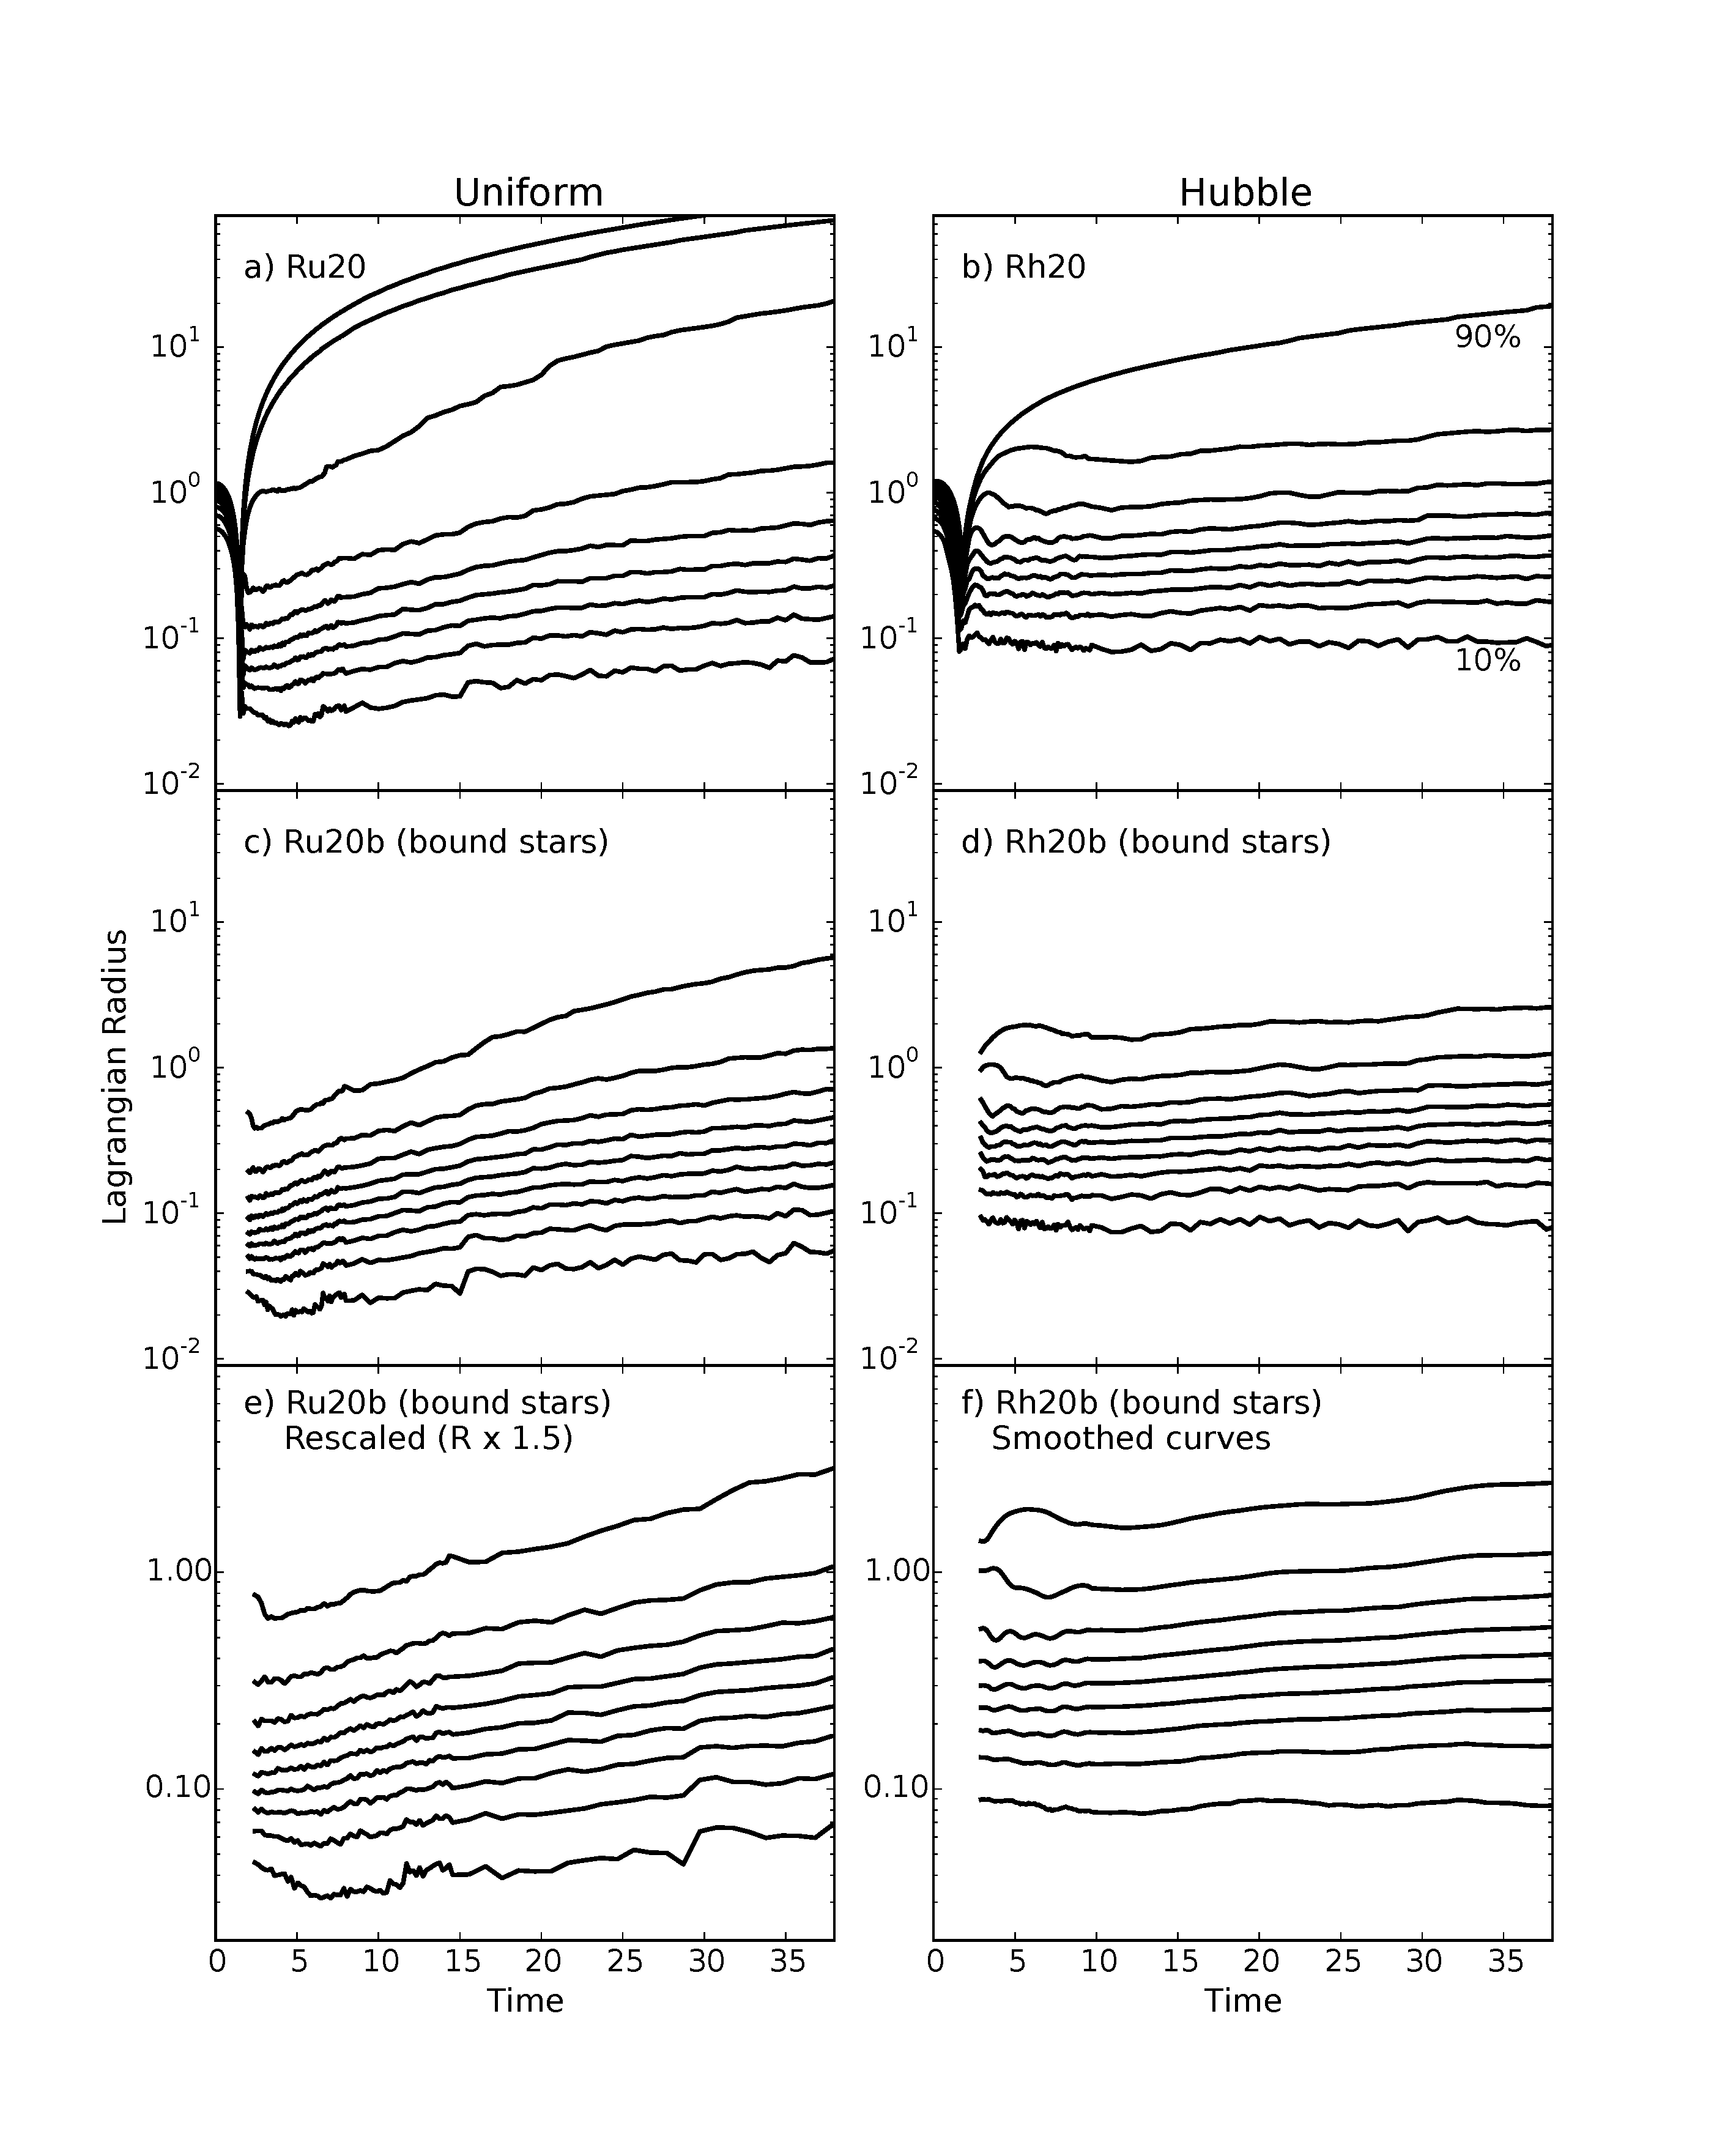
\includegraphics[width=\textwidth]{Figures/3_Lagr_radius}
\caption[Ten-percentile Lagrangian radii over time for HL fragmented and uniform models]{The ten-percentile mass radii (10\% to 90\%) as function of time. Radii and time axis are in H.u, with $t_\Hen = 1 {\rm unit} =  0.13 \Myr$. Left panels show the Uniform model and right panels show the Hubble fragmented models. Panels a and b show the evolution of the whole systems, while panels c and d show the same radii computed for the bound stars only. Panel e shows the Uniform bound model (Ru20b) for which radius and time were rescaled to compensate the difference of initial kinetic energy (see text for details). Panel f shows the same information as panel d with smoothed data. 10\% and 90\% radii are labelled in the top right panel.
%For both, the bottom panel show the bounded systems, with "b" appended to the name,  from which the ejected stars from the initial collapse were removed.
}
\label{Fig:3_Lagr_radius}
\end{center}
\end{figure}


At the bounce, the half-mass radius of the Hubble model is $\approx 4$ times larger than that of the initially uniform sphere at rest (Fig.~\ref{Fig:3_Rhm_global}). The half-mass radii overlap at time $t \approx 15~$H.u. (solid curves) or $t \approx 50~$H.u. (dashed curves). Is the same trend applicable to all Lagrangian radii ? To answer this question we plot on Fig.~\ref{Fig:3_Lagr_radius} the ten-percentile mass radii for the two models. The results are displayed for the two situations including all the stars (top row) or bound stars only (middle row). 

It is striking that the curves show very little evolution at all mass fractions for the case of the Hubble model (see right-hand panels on the figure), whereas all mass shells either contract or expand in time for the uniform one. We have noted how this model should undergo two-body relaxation on a time-scale of $t \approx 320~$H.u. while the innermost 10\% mass shell shows an  indication of \textit{core-collapse} at $t \simeq 5~$H.u.. This is due to the presence of a mass spectrum, the time-scale for core-collapse should be closer to the mass-segregation time-scale,  $t \simeq 25~$H.u.. The remaining difference can be attributed to the smaller total mass (due to the ejecta) and the various assumptions made in section~\ref{Sec:3_Scaling}.

We note here that the two sets of curves reach very similar values at the end of the calculations ($t = 40\, H.u$). A key difference between the two models, therefore, is that the final configuration of the Hubble model is almost identical to what it was at the bounce ; the same simply does not hold in the case of a uniform-density collapse. Furthermore, the Hubble calculation shows no hint of two-body relaxation or core-collapse.
% This raises the possibility that the system properties in the final configuration remain better correlated with those at the on-set of (global) collapse (we return to this point in \S7).

\cite{Caputo2014} and \cite{Theis1999} noted how a non-zero amount of kinetic energy in the {\it initial} configuration alters the  depth of the bounce during collapse. The ratio of half-mass radius at the bounce, to its initial value, is then
\begin{equation}
\frac{R_h}{R_{h,0}} \simeq Q_0 + N^{-1/3}
\end{equation} 
 where $Q_0$ is the virial ratio of the initial configuration \citep[see][Fig.5]{Caputo2014}. We computed the kinetic energy of the  Hubble configuration and found that the internal motion of the clumps means that $Q_0 (Hubble) \simeq 0.02$ for a Salpeter mass function with upper truncation value of $20 \Mo$. With $N = 15k$ stars, the ratio $R_h/R_{h,0} \simeq 0.041$ when $Q_0 = 0$ shifts to $R_h/R_{h,0} \simeq 0.061$ when $Q_o = 0.02$, or a factor close to 1.5. To account for the difference in kinetic energy of the initial configurations, we may therefore rescale the uniform model such that positions are  $ \times 1.5$ and the time unit is $\times (1.5)^{3/2} \simeq 1.84$.
 
  The new configuration would evolve in time in exactly the same way after mapping positions and time to their rescaled values. The result is shown as the bottom row on Fig.~\ref{Fig:3_Lagr_radius}.  Note that we  have blown up the vertical axis to ease comparison between uniform and Hubble models with bound stars only included. The rescaled uniform model is now slightly more extended than before, but overall the final two configurations (at $t = 40~$H.u.) are as close as before rescaling. This demonstrates that  the outcome of the uniform collapse and its comparison with the Hubble model is not sensitive to a small amount of initial kinetic energy. We note that while the ratio $Q_0$ is a free parameter in many setups for collapse calculations, that parameter is fixed internally in the Hubble approach. 










\section{Global mass segregation}
\label{Sec:Segregation} 


To investigate the state of mass segregation in our models, we follow the analysis of \cite{Caputo2014}. The masses are sorted by decreasing values, then subdivided into ten equal-mass bins. This means that the first bin contains the most massive stars. The number of stars in each bin increases as we shift to the following bins, since their mean mass {\it de}creases, and so on until we have binned all the stars. The half-mass radius $R_h$ computed for each bin is then plotted as function of time. In this way the mass segregation unfolds over time: if the stars were not segregated by mass, all radii $R_h$ would overlap. If two sub-populations share the same spatial distribution, their respective $R_h$ will overlap.


\begin{figure}
\begin{center}
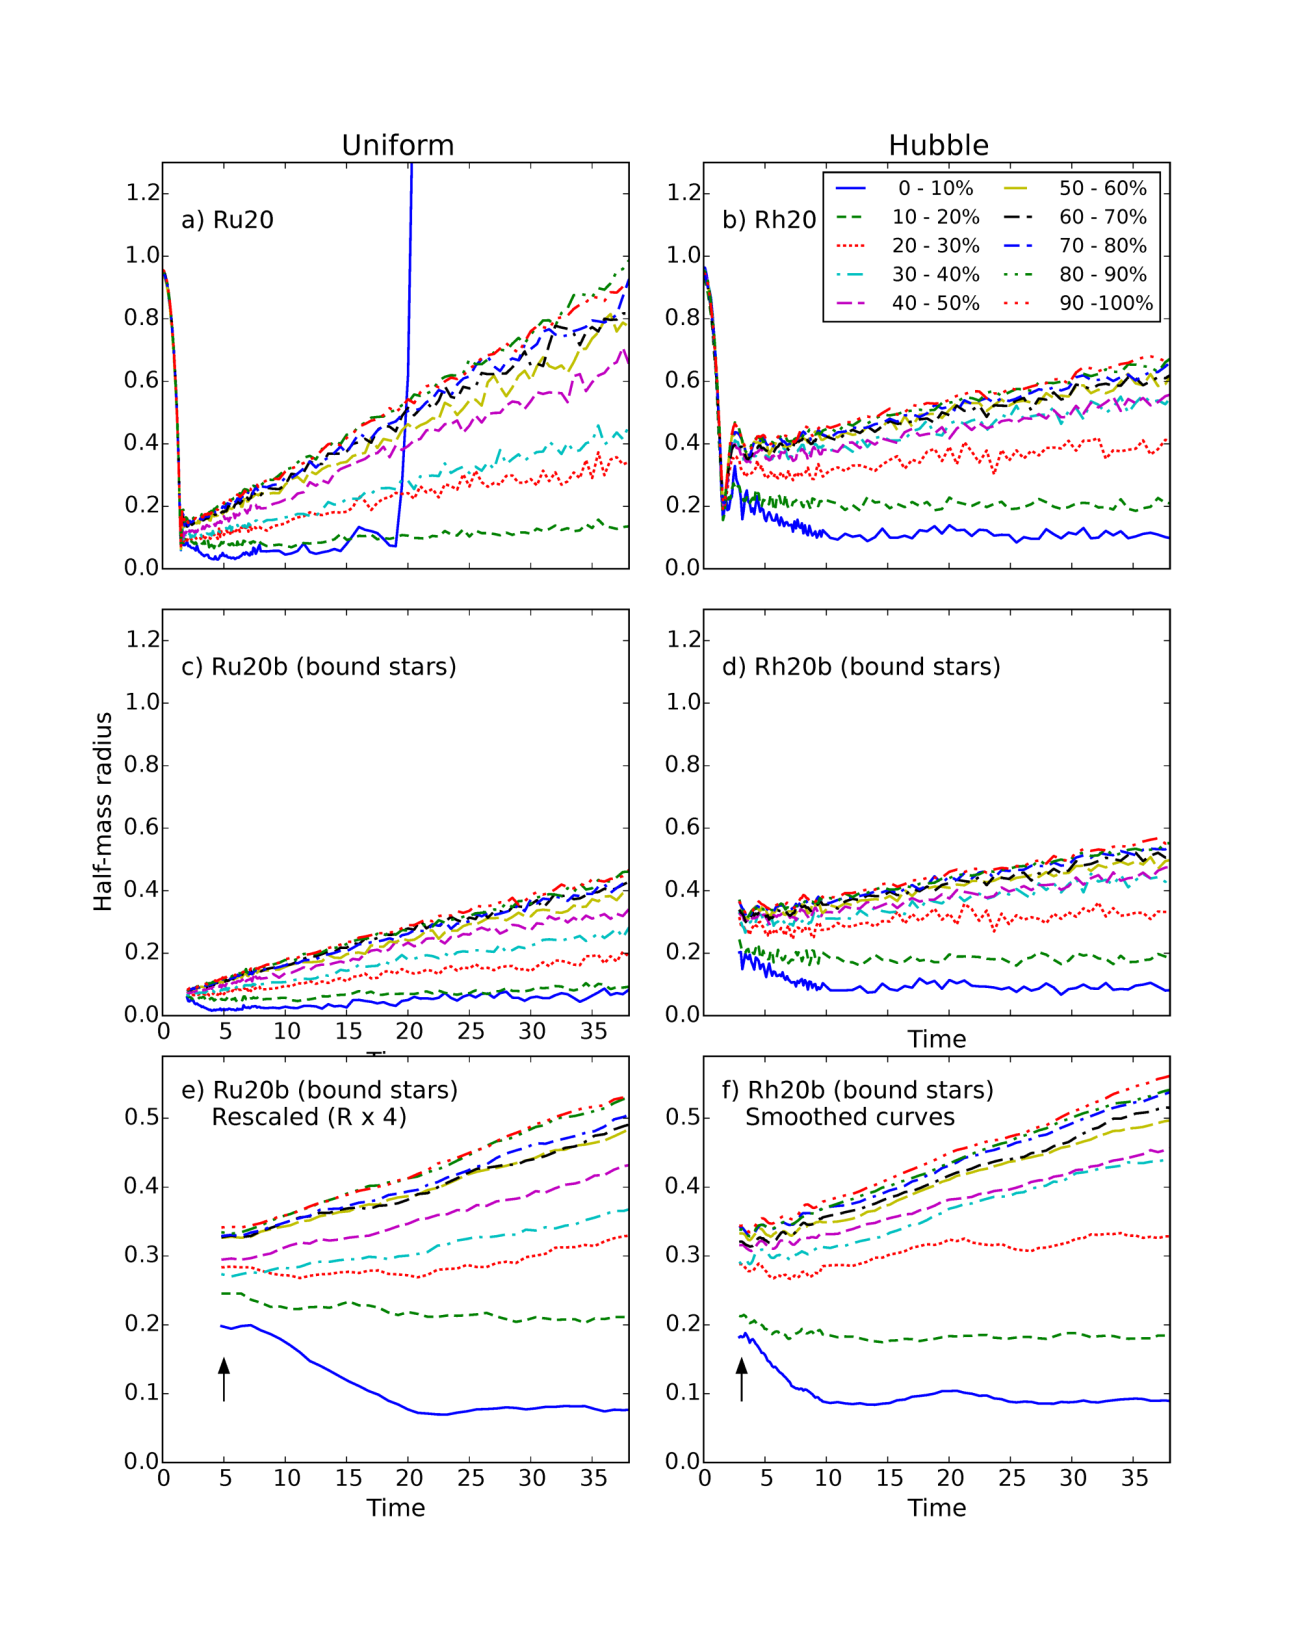
\includegraphics[width=\textwidth,clip=true]{Figures/3_Rhm_segr}
\caption[Mass segregation: half-mass radii over time for mass-selected stars]{Half-mass radii of stars selected by mass as function of time. Each bin identified with 0-10\%, 10-20\% .. 90-100\%, contains ten percent of the total system mass. The stars were sorted by mass in decreasing order, and used to fill each ten-percent mass bin in order. Hence the first ten-percentile contains the most massive stars, the next ten-percentile the second group of massive stars, and so on until the 90-percent bin which contains the least massive stars in the model and is the most populated. Half-mass radius and time are in H.u, with $t_{Henon} = 1\,unit = 0.13 \Myr$. Left panels show the evolution of the Uniform model (Ru20, Ru20b) and right panels do the same for the Hubble model (Rh20, Rh20b). The organization of panels follows the same layout than figure~\ref{Fig:3_Lagr_radius} with a different factor for the rescaling of the uniform system. }
\label{Fig:3_Rhm_segr}
\end{center}
\end{figure}

Figure \ref{Fig:3_Rhm_segr} graphs the results for initially uniform-density and fragmented Hubble models. The layout of the figure is the same as for Fig.~\ref{Fig:3_Lagr_radius}. The violent relaxation phase leads to mass loss for both models and the much more rapid expansion of the half-mass radii of low-mass stars is an indication that most escapers have a lower value of mass.

 Fig.~\ref{Fig:3_Rhm_segr}(c) and (d) graphs $R_h$ for the bound stars of each sub-population. Clearly the initially uniform-density model is more compact early on, but note how the heavy stars sink rapidly to the centre, more so than for the case of the Hubble model. The spread of half-mass radii increases with time for both models, however two-body relaxation in the uniform-collapse calculation is much stronger, so that by the end of the simulations the half-mass radii of the low-mass stars of the respective models are essentially identical. 
 
 Since the low-mass stars carry the bulk of the mass, that means that the two models achieve the same or similar mean surface density by the end of the run. At that time, the heavy stars in the uniform-collapse calculation are clearly more concentrated than in the Hubble run (compare the radii out to $\sim 40\%$ most massive stars). A direct consequence of this is that the {\it color} gradients of the core region of a cluster are much reduced when the assembly history proceeds hierarchically, in comparison with the monolithic collapse. It will be interesting and possibly important in future to compare such models with actual data for young clusters.

Another interesting remark is that the kinematics of the stars within the {\it system} half-mass radius are much different between the two models. For the Hubble calculation, the system half-mass radius, $ \approx 0.43 $ H.u, at $t = 40$ (cf. Fig.\ref{Fig:3_Rhm_segr}d) coincides with the half-mass radius of the $30-40\%$ bin stellar sub-population. All bins up to that range show little or no time-evolution, around the end of the run, which we interpret as efficient retention of these stars by the relaxed cluster. In the case of the uniform-collapse run, the system half-mass radius reaches $\approx 0.33$ H.u., which is significantly larger than the radius for the $30-40\%$ stellar sub-population. For that model, only the bins $0-10\%$ and $10-20\%$ are flat, and all the others increase almost linearly with time. Thus a fair fraction of bright stars deep in the cluster show systematic {\it outward streaming} motion, along with low-mass ones. This brings up the possibility to measure this signature motion through relatively bright stars, originating well inside the cluster half-mass radius. Recall that only post-bounce bound stars where selected to compute $R_h$ on Fig.~\ref{Fig:3_Rhm_segr}(c) and (d) ; the expansion is therefore not driven by escapers (e.g., Fig.~\ref{Fig:3_Rhm_segr}a), but rather through two-body relaxation. On the down side the bright tracers would be short-lived, and this may prove a strong constraint for observational detection.


Given the early dynamical evolution associated with substructured stellar clusters, some observed dense objects may yet be out of equilibrium. We wish to investigate the out-of-equilibrium state of our models just after the collapse. To ease the comparison between the two systems, the same rescaling procedure as for Fig~\ref{Fig:3_Lagr_radius} was applied to the uniform model, only this time the scaling was chosen so that the two clusters have comparable densities after the bounce. Lengths were multiplied by $4$; the time-axis is then scaled up by a factor $(4)^{3/2} = 8$. The result can be seen in panel (e); panel (f) shows a smoothed and zoomed in Hubble model for comparison.



\begin{table}
\caption{Values of half-mass radii and their ratio to that of the most massive stars. The mass categories are labelled X\%-X+10\%, with the percent symbol ommitted for brevity. The results are for the rescaled bound uniform model (rescaled Ru20b) and the bound Hubble model (Rh20b), after the collapse, and before dynamical mass segregation sets in.} \label{Tab:RhmVal}
\begin{center}
\begin{tabular}{l|llllllllll}
Uniform (\%) & 0-10 & 10-20 & 20-30 & 30-40 & 40-50 & 50-60 & 60-70 & 70-80 & 80-90 & 90-100 \\
\hline
Radius   & 0.20 & 0.245 & 0.282 & 0.273 & 0.294 & 0.325 & 0.326 &  0.328 & 0.335 & 0.340 \\
Ratio    & 1 & 1.23 & 1.41 & 1.37 & 1.47  & 1.63 & 1.63 &  1.64 & 1.68 & 1.70 \\

\hline
Hubble (\%) & 0-10 & 10-20 & 20-30 & 30-40 & 40-50 & 50-60 & 60-70 & 70-80 & 80-90 & 90-100 \\
\hline
Radius  &  0.18 & 0.21 & 0.286 & 0.293 & 0.316 & 0.321 & 0.333 & 0.338 & 0.342 & 0.344 \\
 Ratio       & 1 & 1.16 & 1.58 & 1.63 & 1.76  & 1.78  & 1.85 &  1.88 & 1.90 &  1.91 \\
\end{tabular}
\end{center}
\end{table}


%\begin{tabular}{l|llllllllll}
%Uniform  & 0-10\% & 10-20\% & 20-30\% & 30-40\% & 40-50\% & 50-60\% & 60-70\% & 70-80\% & 80-90\% & 90-100\% \\
%\hline
%Radius   & 0.20 & 0.245 & 0.282 & 0.273 & 0.294 & 0.325 & 0.326 &  0.328 & 0.335 & 0.340 \\
%Ratio    & 1.0 & 1.23 & 1.41 & 1.37 & 1.47  & 1.63 & 1.63 &  1.64 & 1.68 & 1.70 \\
%
%\hline
%Hubble  & 0-10\% & 10-20\% & 20-30\% & 30-40\% & 40-50\% & 50-60\% & 60-70\% & 70-80\% & 80-90\% & 90-100\% \\
%\hline
%Radius  &  0.18 & 0.21 & 0.286 & 0.293 & 0.316 & 0.321 & 0.333 & 0.338 & 0.342 & 0.344 \\
% Ratio       & 1.00 & 1.16 & 1.58 & 1.63 & 1.76  & 1.78  & 1.85 &  1.88 & 1.90 &  1.91 \\
%\end{tabular}


We compare the values of the different half-mass radii of the various population before the dynamical mass segregation sets in. This process is clearly visible as the drop of the half-mass radius of the most massive stars during the evolution. We are interested in the segregation which originates from the collapse and is present before this dynamical evolution. Table~\ref{Tab:RhmVal} sums up the values of the half-mass radii taken at $t\sim5$ for both models, both corresponding to the same unevolved post-collapse state (see arrows on panels e and f on Fig~\ref{Fig:3_Rhm_segr}). With on the order of $\sim 100$ stars per bin or more, one estimates roughly a ten-percent standard deviation from random sampling. To measure the \textit{relative} segregation between populations, the table also lists the ratios of each half-mass radius to the one for the most massive stars. 

Both models appear mass segregated (since these ratios are significantly greater than unity). The Hubble model is more segregated, on the whole, albeit in a different way compared to the uniform model. The segregation in that one is more regular and spreads over more mass bins. In the Hubble model, the segregation is much enhanced for the first two mass bins. Such differences in the degree and nature of segregation can be explained by the clumps structure before the collapse. We showed in section \ref{Sec:2_ClumpSegregation} that the clumps were mass segregated with their most massive members being preferentially located at their center. The low membership and mass of most clumps implies that segregation mostly affects the very top of the stellar mass function. This segregation, predominant among massive stars, is then found in the resulting centrally concentrated system, after the collapse, and visible on Fig.~\ref{Fig:3_Rhm_segr}. 

The inheritance of mass segregation was studied by \cite{McMillan2007} for the case of merging Plummer spheres. \cite{Allison2010} furthermore showed that mass segregation in the system as a whole is enhanced for more filamentary  fractal initial conditions (lower dimension, $D$ ; see their Fig. 5). Here our results confirm this observation. Mass segregation is a sensitive function of the initial clumpiness of the system and has immediate bearing on the dynamics of the virialised configuration, since all massive stars are more concentrated in the core.


\section{Concluding remarks}


We have followed \HubLem fragmented models throughout collapse and subsequent dynamical evolution, and compared their structure and mass segregation to cold uniform models. We found fragmented models undergo a softer, shallower collapse than uniform models, due to their irregular spatial distribution and internal kinetic energy. Uniform models eject more than twice as much stars from the system at the bounce due to this deeper collapse and virialize with a 4 times smaller half-mass radius. This high concentration enhances two-body evolution and the uniform systems expand faster than the Hubble models, even when excluding the ejected stars from the system. Interestingly, after 40 H.u, or 6 Myr, both systems achieve approximately the same density and distribution.

Both uniform and fragmented models develop mass-segregation over time, with the low-mass stars being preferentially ejected or diluted. In the end of the simulation, the uniform systems appear slightly more mass-segregated due to their denser configuration and enhanced two-body evolution. However, just after collapse, \HubLem models exhibit a mass segregation mainly affecting the most massive stars. This characteristic is preserved throughout evolution while the segregation seen in uniform models is more spread out in the mass function. This is  a signature of the hierarchical formation, as this ``top-focused" segregation developed in small clumps and was inherited by the whole system. This would enhance colour gradient in the core of real clusters, opening the way for an observational criteria to assess the formation scenario of very young relaxed clusters.






